
To manage the set of in-house and 3rd party RTL,
the \SCARVSOC is split into two layers:

\begin{itemize}[noitemsep]

\item A ``inner" layer, which contains the CPU, local memories, local
    interconnect and any in-house peripherals or subsystems.

\item A ``outer" layer, which wraps the ``inner" layer with vendor specific
    peripherals and subsystems.

\end{itemize}

This separation allows vendor IP and peripherals to be gradually brought
into the inner layer as open-source or in-house alternatives are
found or developed.
Figure \ref{fig:design:soc-blocks} shows the \SCARVSOC block diagram.
The principle components of each layer are shown in 
Table \ref{tab:design:overview:component-layers}.

The inner layer communicates with memory mapped devices in the outer
layer via the AXI4-Lite bus bridge (\SECREF{design:axi-bridge}).
Any data memory request which maps to the bridge is forwarded into
the outer layer.
The outer layer is expected to manage the request and response.
Currently, this is done using a Xilinx AXI4 Interconnect IP.


\begin{figure}
\centering
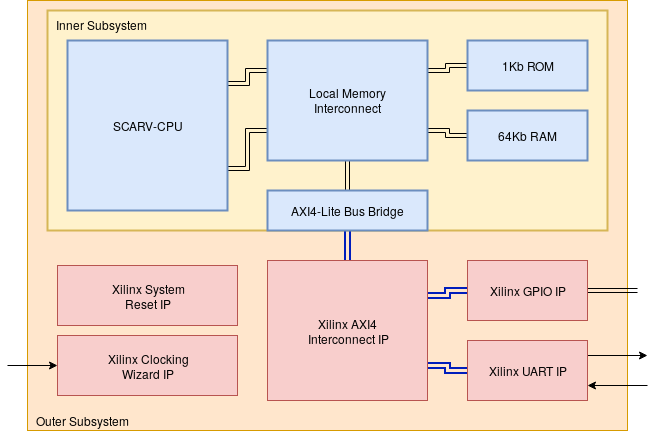
\includegraphics[width=0.8\textwidth]{image/soc-block-diagram.png}
\caption{
Block diagram of the \SCARVSOC, showing the inner subsystem which can be
implemented anywhere, and the Xilinx-specific outer subsystem.
}
\label{fig:design:soc-blocks}
\end{figure}


\begin{table}[H]
\centering
\begin{tabular}{ll}
{\bf Inner Layer}           & {\bf Outer layer} \\ \hline
SCARV-CPU.                  & System clock generation. \\
local memory interconnect.  & System reset control. \\
local RAM and ROM memories. & AXI UART peripheral. \\
AXI4-Lite bus bridge.       & AXI GPIO peripheral.
\end{tabular}
\caption{Main subsystem components of the \SCARVSOC, organised by
the implementation layer they exist in.}
\label{tab:design:overview:component-layers}
\end{table}

